\documentclass[12pt,a4paper]{article}
\usepackage[utf8]{inputenc}
\usepackage{float}
\usepackage{multicol}
\usepackage[a4paper]{geometry}
\usepackage{sectsty}
\geometry{textwidth=480pt, textheight=700pt, noheadfoot, nomarginpar}
\usepackage[square, numbers, comma, sort&compress]{natbib}
\usepackage{graphicx}
\usepackage{microtype}
\usepackage{siunitx}
\usepackage{booktabs}
\usepackage{mathtools}
\usepackage{multicol}
\usepackage{wrapfig}
\usepackage{ragged2e} 
\usepackage{amsmath,amsfonts,amssymb}
\usepackage{url}

\footskip = 40pt

\begin{document}

\numberwithin{equation}{subsection}
\numberwithin{table}{subsection}
\numberwithin{figure}{subsection}

%Title
\begin{minipage}{0.8\textwidth}
\Large \textbf{Artificial Intelligence and Decision Systems}\vspace{0.2cm}\\
Assignment \#2\vspace{0.2cm}\\
\normalsize Professor Luís Manuel Marques Custódio
\end{minipage}
\begin{minipage}{0\textwidth}
\raggedleft

\includegraphics[scale=0.65]{ist_logo.png}
\end{minipage}

\vspace{0.2cm}
\begin{minipage}{0.8\textwidth}
\textbf{Students:} \hspace{0.3cm}
Henrique Carvalho - 70327 \hspace{0.3cm} Gonçalo Ribeiro -  73294

\end{minipage}

\rule{\textwidth}{1pt}


%1st SECTION- ---------------------------------------------
\justify{ 

\section{GSAT}
\subsection{Is the algorithm sound? Is it complete?}
\par \quad 
The algorithm is sound since it only presents valid solutions, that is, a set of values for the variables which satisfies all the CNF sentences. Since GSAT depends partially on random trial to find a solution, it is not complete. It might not find a solution although it exists and may not tell in finite time if there is no solution.


\section{WalkSAT}
\subsection{Is the algorithm sound? Is it complete?}
\par \quad
The algorithm is sound since it only presents valid solutions, that is, a set of values for the variables which satisfies all the CNF clauses. Since WalkSat depends on random trial to find a solution, it is not complete. It might not find a solution although it exists and may not tell in finite time if there is no solution.


\section{DPLL}
\subsection{Is the algorithm sound? Is it complete?}
\par \quad
The algorithm is sound since it only presents valid solutions, that is, a set of values for the variables which satisfies all the CNF clauses. To solve the problem it searches all the sets of values until it finds one that satisfies all clauses or runs out of values to test. Once it runs out of sets of values, it can conclude that there is no solution. This algorithm is complete because if there is a solution it will find it and if there isn't it will infer that in finite time (although it can take really long).



\section{Improving performance of GSAT and WalkSAT}

GSAT and WalkSAT visit neighbours randomly. This means that they can visit the same models several times and make no progress. The performance of these algorithms could be improved by using a tabu list, featuring models already explored, so that the algorithms do not expand those models again.


\section{Performance tests}

From the tests we performed we conclude that the WalkSAT algorithm is faster than GSAT.

We also concluded that DPLL is faster than GSAT and WalkSAT. But is known that the stochastic methods are better for bigger randomly generated problems \cite{dpll_art}. The results go against our expectations and all bibliography consulted. All the generated problems were randomly generated (as stated on the website where we downloaded them). 

On the other hand DPLL is the only complete algorithm of the three, which means it is the only one which can prove that a problem is unsatisfiable.

\subsection{How the tests were made}

We wanted to plot data against the clause/symbol ratios. Nonetheless in the SATLIB website all the clause/symbol ratios are close to 4.5. To solve this problem we wrote scripts to successively remove clauses from the files provided at SATLIB.org until we reached a clause/symbol ratio of 0.5. We ran 1000 different problems (all based on the \texttt{uf20-0*.cnf} files) while varying the number of clauses. Then we took the mean, median and number of satisfied sentences for each clause/symbol ratio and we made the plots in this report.

\begin{figure}[htbp]
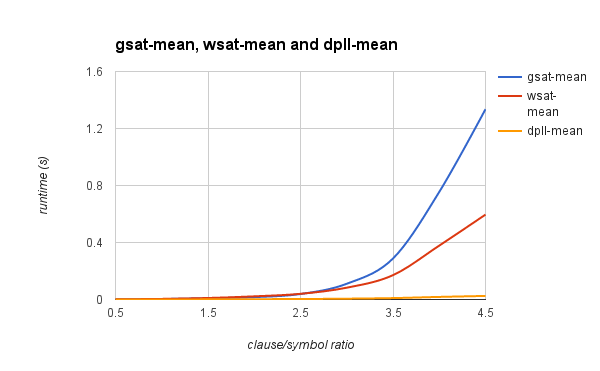
\includegraphics[width=\textwidth]{CS_mean}
\end{figure}

\begin{figure}[htbp]
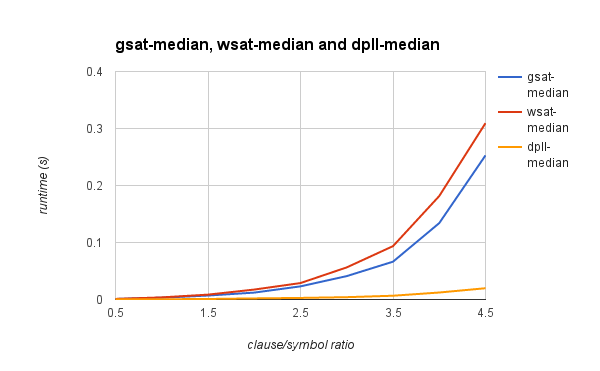
\includegraphics[width=\textwidth]{CS_median}
\end{figure}

\begin{figure}[htbp]
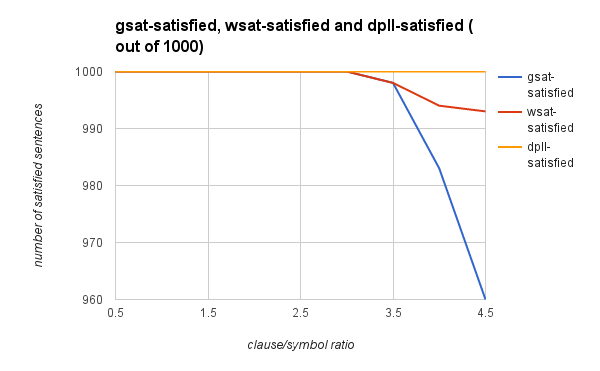
\includegraphics[width=\textwidth]{CS_satisfied}
\end{figure}


\pagebreak
\begin{thebibliography}{9} 
\bibitem{dpll_art} 
\emph{WalkSAT as an Informed Heuristic to DPLL in SAT Solving}
\url{https://www.cs.umd.edu/~jonf/publications/Ferris_WalkSATAsAnInformedHeristicToDPLLInSATSolving_WeldAICourse2005.pdf}


\end{thebibliography}


\end{document}